\documentclass[12pt]{article}

\usepackage{sbc-template}
\usepackage{graphicx}
\usepackage{url}
\usepackage[utf8]{inputenc}
\usepackage{booktabs}
\usepackage{amsmath,amssymb}
\usepackage{subcaption}

\sloppy

\title{Predicting Cross-Repository Reuse and Diffusion of AI Agent Skills: A Multimodal Empirical Study on GitHub\footnote{Replication package, dataset access, and 1-click Google Colab notebook: \url{https://github.com/podorize/skillreuse}.}}

\author{Pedro Odorize\inst{1}}

\address{Instituto de Inform\'atica -- Universidade Federal do Rio Grande do Sul (UFRGS)\\
  Porto Alegre, RS -- Brazil
  \email{pedro.odorize@inf.ufrgs.br}
}

\begin{document}

\maketitle

\begin{abstract}
Modular skill specifications (\texttt{SKILL.md}) standardise agent capabilities, yet drivers of cross-repository reuse remain unknown. Analyzing 200,000 skills across 72,376 repositories under zero-leakage grouped splits, we show that tree models suffer shortcut learning, while regularized linear models generalize reliably (0.6188 test ROC-AUC). Threshold tuning ($t^*=0.21$) boosts $F_1$-score by $+372\%$, recovering 49.82\% of viral skills. Interpretability reveals Three Pillars of Reuse: structural canonicity, host ecosystems, and prompt contracts.
\end{abstract}

\section{Introduction}

The rapid transition from conversational Large Language Models (LLMs) to autonomous agentic architectures has introduced a fundamentally new artifact to software engineering: \emph{agent skills}. Popularized by modern developer environments such as Google Antigravity, Claude Code, and GitHub Copilot Workspace, agent capabilities are increasingly encapsulated in modular Markdown specifications, conventionally titled \texttt{SKILL.md}. These files combine structured metadata, natural language operational contracts, executable tool declarations, parameter constraints, and contextual few-shot demonstrations.

In traditional software engineering, component reuse has long served as a primary catalyst for developer productivity, software quality, and architectural convergence \cite{haefliger2008code,lopes2017dejavu}, mediated by mature package registries (e.g., npm, PyPI) that enforce semantic versioning, dependency tracking, and static verification. In stark contrast, agent skills currently lack centralized package management \cite{gitskills2027}. Instead, skills diffuse organically via decentralized, peer-to-peer directory copying across open-source repositories. This package-manager vacuum introduces three critical software engineering challenges:
\begin{enumerate}
    \item \textbf{Authoring Uncertainty (The Engineering Blind Spot)}: Unlike traditional programming where compilers and linters enforce structural sanity, prompt engineers author skills in the dark, lacking empirical guidance on which formatting conventions, structural schemas, or contractual constraints ensure skill robustness and reliable agent execution.
    \item \textbf{Uncurated Discovery (The Commons Dilemma)}: Autonomous agents searching public repositories cannot reliably distinguish mature, generalizable capabilities from transient, single-use drafts.
    \item \textbf{Supply-Chain Security and Malicious Propagation}: Because skills instruct language models to execute terminal commands, run bundled scripts, and access network endpoints, viral unvetted skills pose latent supply-chain attack vectors.
\end{enumerate}

To address these challenges, this paper formulates the study of skill characteristics as a supervised machine learning classification problem. Crucially, we treat cross-repository persistence---the deliberate copying and retention of an exact cryptographic skill payload across distinct Git repositories---as an \emph{observational proxy} for community adoption and perceived utility. While observational reuse does not guarantee absolute functional robustness, predicting reuse provides an empirical foundation to extract actionable engineering patterns. Scientifically, this supervised formulation subjects authoring hypotheses to the acid test of out-of-distribution generalization on unseen codebases \cite{shmueli2010explain}; operationally, it provides the empirical engine for two practical developer tools:
\begin{itemize}
    \item \textbf{An Agent Skill Authoring Linter}: Embedded in developer IDEs (e.g., pre-commit hooks or VS Code plugins) to provide real-time diagnostic feedback on structural conformity and contractual completeness before committing;
    \item \textbf{An Ecosystem Ranking Prior}: Designed for decentralized skill search engines (Learning-to-Rank pipelines) to prioritize well-specified, modular skills in autonomous agent capability discovery.
\end{itemize}

Specifically, we investigate two foundational research questions:
\begin{itemize}
    \item \textbf{RQ1 (Predictability of Skill Adoption)}: \emph{To what extent can intrinsic file attributes (structural syntax and instructional text) and external repository context distinguish cross-repository adopted skills ($\ge 2$ repositories) from isolated singletons in previously unseen codebases?}
    \item \textbf{RQ2 (Drivers of Ecosystem Diffusion Scale)}: \emph{Conditional on successful adoption, what architectural, syntactic, and ecosystem factors govern the scale of skill diffusion (differentiating small-scale paired sharing from massive viral diffusion across $10+$ repositories)?}
\end{itemize}

Mining a deduplicated dataset of 200,000 unique skills across 72,376 GitHub repositories under a zero-leakage grouped partition ($160,000$ train / $40,000$ test), our core contributions are:
\begin{itemize}
    \item \textbf{First Large-Scale Empirical Benchmark on Agent Skills}: We provide the first comprehensive study, public dataset ($N=200,000$), and zero-leakage grouped evaluation benchmark on 14,568 unseen repositories, establishing a reproducible foundation for empirical research on AI agent components.
    \item \textbf{Empirical Principles of Skill Adoption (The Three Pillars)}: Using standardized Odds Ratios and game-theoretic SHAP attributions, we demonstrate that task domain does not govern skill adoption; rather, reuse is driven by structural canonicity ($+87\%$), host modular ecosystems, and formal prompt specification contracts. Furthermore, syntactic frontmatter validation enables the model to recover 49.82\% of viral superpropagators.
    \item \textbf{Actionable Foundations for Developer Tooling}: We translate our empirical parameters and probability-calibrated thresholds into concrete decision rules that directly power two practical software tools: an \emph{Authoring Linter} for developer IDEs and an \emph{Ecosystem Ranking Prior} for decentralized skill discovery.
\end{itemize}

\section{Related Work}

\subsection{Software Reuse and Code Duplication in MSR}
Component and code reuse is a cornerstone of empirical software engineering. Seminal investigations by Mockus et al. \cite{mockus2002two} and Haefliger et al. \cite{haefliger2008code} explored developer motivations and architectural drivers of component adoption in open-source projects. In large-scale repository mining, Lopes et al. \cite{lopes2017dejavu} conducted the monumental D{\'e}j{\`a}Vu study, revealing massive file-level code duplication across millions of GitHub repositories. While prior literature focused on procedural code, package dependencies, and binary libraries, modern AI software engineering introduces a fundamentally novel entity: \emph{executable markdown prompt specifications}. Our study extends empirical software reuse research into the emerging domain of natural language agent assets.

\subsection{Tool Specifications and LLM Agent Skills}
Autonomous LLM agents rely on modular skill declarations to interact with external environments. Foundational frameworks including Toolformer \cite{schick2023toolformer}, HuggingGPT \cite{shen2023hugginggpt}, ReAct \cite{yao2023react}, and ToolLLM \cite{qin2023toolllm} demonstrate that LLMs execute complex planning when supplied with concise, structured tool descriptions. More recently, standardization initiatives such as the Model Context Protocol (MCP) and Google Antigravity have formalized \texttt{SKILL.md} as an open schema for agent capabilities. While recent mining efforts have analyzed intra-repository prompt changes in LLM applications \cite{tafreshipour2025prompting}, the organic cross-repository diffusion of modular, folder-based agent skill specifications without package managers has emerged as an open empirical challenge \cite{gitskills2027}. To the best of our knowledge, this work presents the first large-scale predictive investigation addressing this challenge across the GitHub ecosystem.

\subsection{Shortcut Learning, Group Leakage, and Generalization}
Machine learning models trained on observational software data are notoriously susceptible to \emph{shortcut learning} and \emph{Clever Hans} artifacts \cite{geirhos2020shortcut,lapuschkin2019unmasking}. In software analytics, Kaufman et al. \cite{kaufman2012leakage} and Saeb et al. \cite{saeb2017need} showed that when samples from the same project or subject appear across training and validation splits, models inadvertently memorize cluster-level identifiers rather than generalizable problem features. Roberts et al. \cite{roberts2017cross} formalized grouped cross-validation as an absolute prerequisite for hierarchical data structures. In this paper, we systematically analyze this failure mode within GitHub repository hierarchies, contrasting non-linear tree partitioning with regularized linear representations.

\section{Dataset and Problem Formulation}

\subsection{Unit of Analysis, Dataset Access, and Deduplication Protocol}
The target population comprises all open-source repositories on GitHub declaring agent skill specifications, collected from the GitSkills public benchmark \cite{gitskills2027}.\footnote{The complete dataset, preprocessed matrix caches, and code are publicly accessible for download at \url{https://github.com/podorize/skillreuse}.} The atomic unit of analysis is a unique normalized content payload of a \texttt{SKILL.md} file, uniquely identified by its cryptographic SHA-256 digest (\texttt{content\_hash}). Content deduplication is performed strictly prior to dataset splitting, ensuring that identical copies across different forks or directories do not inflate sample counts artificially.

\subsection{Dual-Target Formulation}
We formulate the investigation around two complementary prediction targets:
\begin{enumerate}
    \item \textbf{Binary Reuse ($y \in \{0, 1\}$)}: Defined as $y = 1$ if the exact \texttt{content\_hash} is observed in $\ge 2$ distinct GitHub repositories, and $y = 0$ if it is a singleton observed in exactly one repository.
    \item \textbf{Conditional Intensity ($y_{\text{int}} \in \{0, 1, 2, 3\}$)}: Applicable strictly conditional on $y = 1$, representing the scale of ecosystem diffusion:
    \begin{itemize}
        \item Class 0 ($2$ repositories): Small-scale paired sharing ($56.3\%$ of reused skills).
        \item Class 1 ($3$--$4$ repositories): Moderate diffusion ($23.5\%$).
        \item Class 2 ($5$--$9$ repositories): Broad adoption ($11.7\%$).
        \item Class 3 ($10+$ repositories): Massive viral diffusion ($8.5\%$).
    \end{itemize}
\end{enumerate}

\subsection{Exploratory Data Analysis (EDA)}
Prior to model training, we conducted systematic exploratory data analysis across the $200,000$ extracted skills, summarized in Table~\ref{tab:eda_summary}:
\begin{itemize}
    \item \textbf{Target Distribution and Extreme Class Imbalance}: Exactly $16.20\%$ ($32,397$ skills) are reused across $\ge 2$ repositories, whereas $83.80\%$ ($167,603$ skills) exist as singletons. Among reused skills, the distribution follows a severe Pareto-like decay: $56.3\%$ diffuse to only 2 repositories, while only $8.5\%$ achieve viral diffusion ($\ge 10$ repositories).
    \item \textbf{Outlier Profiles and Heavy-Tailed Distributions}: Continuous repository metrics exhibit extreme positive skewness spanning multiple orders of magnitude: repository stars range from $0$ to over $52,000$ (median: $3$, interquartile range: $1$--$24$), and commit counts range from $1$ to over $100,000$. Similarly, skill file lengths vary from minimal stubs ($34$ characters) to verbose workflow manuals ($> 45,000$ characters).
    \item \textbf{Missingness and Anomaly Screening}: Structural textometrics exhibited zero missing values across all $200,000$ records. Repository-level categorical variables contained missing values for unclassified programming languages ($12.4\%$) and undeclared open-source licenses ($18.1\%$), which were systematically mapped to dedicated \texttt{'Unknown'} categorical bins rather than dropped.
\end{itemize}

\begin{table}[ht]
\centering
\caption{Exploratory Data Analysis (EDA): Summary statistics, class distributions, and feature modalities across the 200,000 deduplicated agent skills.}
\label{tab:eda_summary}
\small
\begin{tabular}{llcc}
\toprule
\textbf{Category} & \textbf{Metric / Attribute} & \textbf{Count / Value} & \textbf{Proportion} \\
\midrule
\textbf{Population} & Total Unique Skills ($N$) & $200,000$ & $100.0\%$ \\
 & Unique GitHub Repositories & $72,376$ & --- \\
\midrule
\textbf{Binary Reuse Target ($y$)} & Singleton ($y = 0$, 1 repository) & $167,603$ & $83.80\%$ \\
 & Reused ($y = 1$, $\ge 2$ repositories) & $32,397$ & $16.20\%$ \\
\midrule
\textbf{Diffusion Intensity ($y_{\text{int}}$)} & Class 0 (Paired sharing: 2 repos) & $18,243$ & $56.31\%$ \\
 & Class 1 (Moderate: 3--4 repos) & $7,606$ & $23.48\%$ \\
 & Class 2 (Broad: 5--9 repos) & $3,782$ & $11.67\%$ \\
 & Class 3 (Viral superpropagators: $\ge 10$) & $2,766$ & $8.54\%$ \\
\midrule
\textbf{Structural Modality} & Valid YAML Frontmatter Header & $82,419$ & $41.21\%$ \\
 & Canonical Skill Path (\texttt{location\_class}) & $56,792$ & $28.40\%$ \\
 & Content Length (characters) & Median: $1,420$ & IQR: $580$--$3,650$ \\
 & Markdown Heading Count & Median: $4$ & IQR: $2$--$8$ \\
\midrule
\textbf{Repository Modality} & Repository Star Count & Median: $3$ & IQR: $1$--$24$ (Max: $52,140$) \\
 & Repository Commit Count & Median: $184$ & IQR: $35$--$940$ (Max: $>100\text{k}$) \\
 & Primary Host Languages & HTML, Python, JS, Svelte & $64.8\%$ of population \\
\bottomrule
\end{tabular}
\end{table}

\subsection{Construct Validity: Cross-Repository Reuse as an Empirical Quality Proxy}
A fundamental conceptual question in empirical software mining is whether cross-repository reuse reflects genuine implementation quality or mere popularity bias. In traditional software ecosystems, poorly designed packages occasionally accumulate downloads through first-mover advantages or social virality. In the context of agent skills, the gold-standard measure of intrinsic quality would ideally be dynamic execution success rate (e.g., benchmark pass-rates across real-world SWE-bench or GAIA tasks). However, executing thousands of LLM inference queries across 200,000 heterogeneous skills is computationally and economically prohibitive ($> \$100,000$ in commercial API costs).

Consequently, following established MSR methodologies \cite{mockus2002two,haefliger2008code,lopes2017dejavu}, we adopt cross-repository persistence---the deliberate copying and retention of an exact cryptographic skill payload across multiple independent Git commit trees---as an observational proxy for perceived utility and reusability. While an individual project may commit a singleton skill as an ephemeral experiment, repeated cross-project adoption indicates that independent engineering teams judged the artifact sufficiently robust and generalizable to integrate into their autonomous workflows.

\subsection{Methodological Rationale: Predictive Modeling as an Empirical Engine}
A fundamental methodological decision in this investigation is formulating the study of skill characteristics as a supervised predictive modeling problem, rather than relying solely on descriptive statistics or classical bivariate hypothesis testing (e.g., Mann-Whitney $U$ or $t$-tests). This design is grounded in four core principles of empirical software engineering and statistical science:
\begin{enumerate}
    \item \textbf{Mitigating the Large-Sample Fallacy}: With a population of $N = 200,000$ skills, traditional null-hypothesis significance testing suffers from the ``large sample problem'' \cite{lin2013too}: standard errors shrink toward zero ($\text{SE} \propto 1/\sqrt{N}$), causing virtually any negligible or spurious difference to yield extreme statistical significance ($p < 10^{-15}$). Focusing strictly on out-of-sample predictive power provides an objective empirical filter that rejects statistically significant yet practically meaningless attributes.
    \item \textbf{Controlling for Multivariate Confounding}: In decentralized software ecosystems, artifacts are shaped by complex multimodal interactions across repository popularity, structural syntax, and instructional wording. Bivariate comparisons risk severe omitted variable bias and Simpson's Paradox. In accordance with Breiman's algorithmic modeling paradigm \cite{breiman2001statistical}, supervised models evaluate the joint marginal contribution of candidate features while holding contextual repository variables constant.
    \item \textbf{Out-of-Distribution Generalization as the Scientific Acid Test}: Following Shmueli's foundational distinction between explanatory and predictive modeling \cite{shmueli2010explain}, explanatory post-hoc correlations fit to historical data often fail when exposed to unseen environments. By enforcing zero-leakage grouped cross-validation and evaluating on 14,568 untouched external repositories, predictive accuracy serves as the ultimate test of whether the identified characteristics capture genuine, generalizable engineering principles \cite{roberts2017cross,menzies2010defect}.
    \item \textbf{From Predictive Power to Actionable Analytics}: In software analytics, predictive models are rarely deployed merely as black-box oracles; their primary utility lies in what they reveal about the software engineering process \cite{menzies2010defect,tantithamthavorn2020code}. By coupling regularized linear modeling with standardized Odds Ratios and game-theoretic SHAP attributions \cite{lundberg2017unified,molnar2020interpretable}, the predictive framework directly translates model parameters into actionable authoring linters and ecosystem ranking priors.
\end{enumerate}

\subsection{Leakage-Free Grouped Stratified Partitioning}
Skills originating within the same GitHub repository share identical contextual variables (e.g., star count, commit count, sibling files). Naive random splitting would permit algorithms to identify repository membership, causing severe data leakage. 

To eliminate this vulnerability, we partition the dataset using \texttt{StratifiedGroupKFold}, setting the representative repository identifier (\texttt{representative\_repo\_id}) as the grouping factor, and the joint target stratum (\texttt{split\_stratum}) as the stratification factor. As documented in our verified metadata manifest (\texttt{final\_feature\_manifest.json}):
\begin{itemize}
    \item \textbf{Training Partition}: $160,000$ unique skills across $57,808$ repositories.
    \item \textbf{External Test Partition}: $40,000$ unique skills across $14,568$ repositories.
    \item \textbf{Repository Overlap}: \textbf{Exactly 0} ($\text{Train} \cap \text{Test} = \emptyset$).
    \item \textbf{Target Prevalence}: Preserved at exactly $16.20\%$ in both training ($25,918 / 160,000$) and test ($6,479 / 40,000$).
\end{itemize}

\subsection{Data Preprocessing and Multimodal Feature Engineering}
To prepare the heterogeneous raw data for algorithmic learning while rigorously guarding against leakage, we constructed automated, scikit-learn compatible preprocessing pipelines:
\begin{itemize}
    \item \textbf{Continuous Standardization}: Continuous numerical attributes (e.g., character length, line counts, commit counts, star counts) are transformed via \texttt{StandardScaler}. Scaler parameters (mean and variance) are computed strictly on the training partition of each split and applied out-of-sample.
    \item \textbf{Categorical Encoding}: Discrete nominal attributes (\texttt{location\_class}, \texttt{filename}, \texttt{repo\_language}, and \texttt{repo\_license}) are encoded via \texttt{OneHotEncoder(handle\_unknown='ignore')}, mapping unseen test levels to zero vectors without breaking pipeline integrity.
    \item \textbf{Missing Value Imputation}: Missing values in categorical indicators are encoded with dedicated \texttt{'Unknown'} tokens, while numeric missingness is imputed via median imputation (\texttt{SimpleImputer(strategy='median')}).
    \item \textbf{Textual Representation and Supervised $\chi^2$ Screening}: For prompt content, we compute sublinear TF-IDF vectors ($1 + \log(\text{tf})$) over unigrams and bigrams ($\text{min\_df}=5, \text{max\_df}=0.95$). To combat the curse of dimensionality ($50,000$ features), we apply supervised univariate $\chi^2$ screening (\texttt{SelectKBest(chi2, k=100)}). The screening is fitted exclusively on each training fold, selecting the 100 terms with highest statistical dependence with the reuse target.
\end{itemize}
In total, the raw multimodal space comprises 46 structural attributes, 97 repository context variables, and 50,000 textual n-grams, condensed to a 243-dimensional screened hybrid space.

\paragraph{Class Imbalance Strategy: Natural Calibration vs. Synthetic Resampling}
A pivotal design decision is addressing the $16.20\%$ positive prevalence without corrupting posterior probabilities. Rather than generating synthetic points (e.g., SMOTE) or performing severe undersampling---both of which distort empirical class proportions, degrade probability calibration, and artificially inflate Brier Score losses---we preserve the authentic population distribution during gradient optimization. By keeping posterior probabilities uncorrupted, the model achieves near-ideal calibration reliability (Brier Score Loss $= 0.1323$). We then address the asymmetric decision cost in the post-training inference phase via cost-sensitive decision threshold optimization ($t^* = 0.21$).

\section{Experimental Methodology}

\subsection{Algorithmic Spot-Checking \& Inductive Bias Analysis}
In accordance with rigorous empirical machine learning methodology, we initially conducted spot-checking across diverse inductive learning biases:
\begin{enumerate}
    \item Non-linear, non-parametric tree ensembles: Histogram Gradient Boosted Decision Trees (\texttt{HistGradientBoostingClassifier}) and Random Forests.
    \item Parametric regularized linear models: Logistic Regression with $L_2$ penalty.
    \item Non-parametric instance/tree baselines: Individual Decision Trees and Nearest Neighbors.
    \item Zero-rule probabilistic heuristic: Dummy Stratified Classifier.
\end{enumerate}

\paragraph{Primary Evaluation Criteria}
Following course guidelines, we formally designate \textbf{grouped cross-validation ROC-AUC} as our \textbf{primary discriminative metric for model selection}, as it rigorously benchmarks the algorithm's global ranking capability across entirely unseen repositories independent of decision thresholds. In parallel, we establish the \textbf{$F_1$-score at the calibrated operating threshold ($t^*=0.21$)} as our \textbf{primary operational utility metric}, directly quantifying practical precision-recall trade-offs for real-world software engineering linters.

\begin{figure}[!htbp]
    \centering
    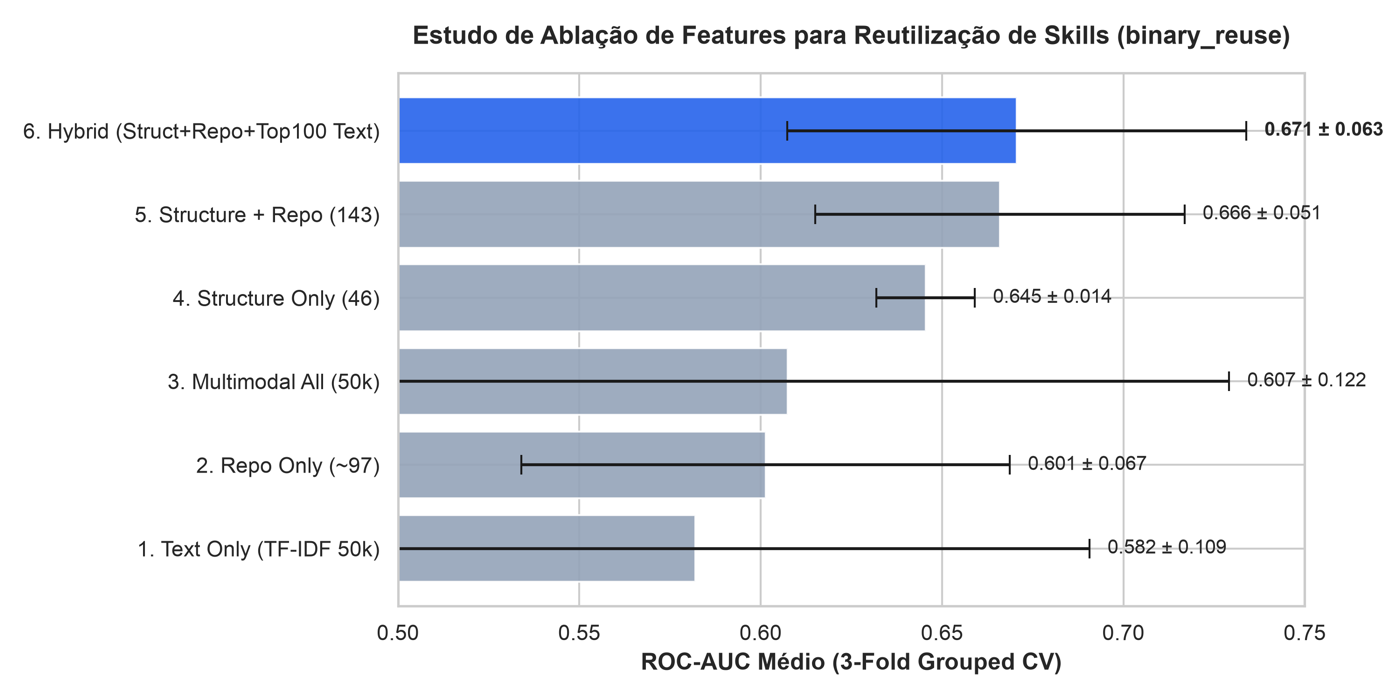
\includegraphics[width=0.75\textwidth]{figures/ablation_roc_auc_comparison.png}
    \caption{Cross-validation ROC-AUC across multimodal ablation configurations under 3-Fold StratifiedGroupKFold.}
    \label{fig:ablation_roc}
\end{figure}

\subsubsection{Unmasking the Shortcut Learning Artifact}
Under standard randomized $I.I.D.$ cross-validation, Histogram Gradient Boosting achieved an extraordinary ROC-AUC of $\mathbf{0.8514}$. However, inspecting the decision tree split criteria revealed an immediate pathology:
\begin{itemize}
    \item Because multiple skills shared the exact same continuous values for \texttt{sibling\_bytes}, \texttt{commit\_count}, and \texttt{repo\_stars}, the tree algorithms recursively partitioned continuous feature space to isolate individual repository IDs present in both training and test folds.
    \item When evaluated under strict grouped cross-validation (\texttt{StratifiedGroupKFold}) on 100\% unseen repositories, tree ensembles suffered a \textbf{catastrophic generalization collapse}, with ROC-AUC plummeting to $\mathbf{0.48 \sim 0.62}$.
    \item Conversely, $L_2$-regularized Logistic Regression restricts hypothesis complexity to a global monotonic hyperplane $\sigma(w^T x + b)$. Unable to isolate arbitrary continuous feature slices, the linear model achieved robust, stable out-of-fold generalization ($0.6706$ ROC-AUC).
\end{itemize}
Consequently, regularized linear modeling was selected as the foundational architecture for all subsequent analyses.

\subsection{Multimodal Ablation Design}
To quantify the exact marginal contribution of each modality, we configured 6 systematic ablation pipelines evaluated under 3-Fold \texttt{StratifiedGroupKFold}:
\begin{itemize}
    \item \textbf{\texttt{text\_only}}: 50,000 sublinear TF-IDF n-grams exclusively.
    \item \textbf{\texttt{repo\_only}}: 97 repository context variables exclusively.
    \item \textbf{\texttt{structure\_only}}: 46 structural and textometric variables exclusively.
    \item \textbf{\texttt{structure\_and\_repo}}: 143 combined tabular structural and repository variables.
    \item \textbf{\texttt{all}}: 50,150 raw multimodal features (TF-IDF + Structure + Repo).
    \item \textbf{\texttt{hybrid\_screened}}: 143 tabular features + Top-100 textual n-grams screened via supervised univariate $\chi^2$ feature selection fitted strictly on each training fold.
\end{itemize}

\subsection{Probability Calibration and Threshold Optimization}
Due to the class imbalance ($16.20\%$ positive prevalence), standard decision thresholds ($t = 0.50$) introduce severe decision bias. Rather than artificially distorting posterior probabilities during gradient optimization (e.g., via heuristic class reweighting), we preserve natural probability calibration and optimize the operational decision threshold $t^*$.

Using out-of-fold predictions on the 160,000 training samples, we evaluate calibration reliability via Brier Score Loss and sweep 86 operational thresholds ($t \in [0.05, 0.90]$ with step $0.01$). The optimal threshold $t^*$ is selected to maximize the macro-operational $F_1$-score on the training split, and subsequently \textbf{strictly frozen} prior to any external test evaluation.

\subsection{Hypothesis Space Exploration: Benchmarking Diverse Inductive Biases}
To ensure that our methodological choices are rigorously grounded in statistical machine learning, we investigated whether the solution space was exhausted under our computational budget. Rather than arbitrarily selecting a single model family, we systematically benchmarked five diverse inductive biases across the 243-feature hybrid representation under identical 3-Fold \texttt{StratifiedGroupKFold} splitting ($N=160,000$ training instances):
\begin{enumerate}
    \item \textbf{Convex Linear Anchor ($L_2$-Regularized Logistic Regression)}: Restricts hypotheses to a global monotonic separating hyperplane $\sigma(w^T x + b)$ solved via L-BFGS, yielding exact closed-form Odds Ratios ($\text{OR} = e^\beta$).
    \item \textbf{Sparse and Shrinkage Regularization (ElasticNet via SAGA/SGD)}: Blends $L_1$ and $L_2$ penalties ($50\%$ mixing ratio) to test whether automated sparse feature elimination improves out-of-fold discriminative power.
    \item \textbf{Multi-Layer Perceptron (2-Layer Neural Network)}: Evaluates universal continuous non-linear function approximation through dense compositions (64 and 32 hidden units, ReLU activations, $L_2$ weight decay $\alpha=0.01$, and validation early stopping).
    \item \textbf{Constrained Tree Ensemble (Anti-Shortcut GBDT)}: Explores recursive orthogonal axis partitioning via Histogram Gradient Boosting with aggressive anti-shortcut hyperparameter controls (\texttt{min\_samples\_leaf=200}, \texttt{max\_depth=3}, $\eta=0.05$, 60 estimators) to restrict continuous feature isolation.
    \item \textbf{Heterogeneous Multi-Paradigm Blend (Stacking)}: Combines diverse hypothesis classes through soft convex probability voting ($0.50 \cdot \text{Linear} + 0.25 \cdot \text{GBDT} + 0.25 \cdot \text{MLP}$).
\end{enumerate}

\subsection{Reproducibility Protocol and Rapid Verification}
In strict adherence to experimental reproducibility standards, all random states across data partitioning, model initialization, and sub-sampling are locked to a single deterministic seed (\texttt{seed=42}). To eliminate computational bottlenecks during independent peer review without sacrificing dataset fidelity ($N=200,000$), all preprocessed sparse matrices (one-hot categorical matrices, scaled textometrics, and sublinear TF-IDF arrays) are serialized in compressed SciPy \texttt{.npz} format ($61$~MB total, version-controlled directly within the repository). A dedicated lightweight reproduction script (\texttt{gitskills\_reuse.reproduce}) trains the champion pipeline, evaluates external test metrics, and exports verification logs in approximately $45$ to $200$ seconds. Furthermore, an interactive, zero-setup Google Colab notebook is provided at \url{https://colab.research.google.com/github/podorize/skillreuse/blob/main/notebooks/reproduce_in_colab.ipynb}, with the complete replication package hosted at \url{https://github.com/podorize/skillreuse}.

\section{Empirical Results and Analysis}

\subsection{Multimodal Ablation Findings}
Table~\ref{tab:ablation_cv} presents the cross-validation performance across the 6 ablation configurations on the 160,000 training instances.

\begin{table}[ht]
\centering
\caption{Cross-Validation performance across ablation suites (3-Fold StratifiedGroupKFold).}
\label{tab:ablation_cv}
\small
\begin{tabular}{lcccc}
\toprule
\textbf{Configuration} & \textbf{Feature Space} & \textbf{ROC-AUC} & \textbf{PR-AUC} & \textbf{Intensity Macro $F_1$} \\
\midrule
\texttt{text\_only} & $50,000$ TF-IDF & $0.5818 \pm 0.1086$ & $0.2230 \pm 0.0422$ & $0.2505 \pm 0.0384$ \\
\texttt{repo\_only} & $\sim 97$ Repo & $0.6006 \pm 0.0673$ & $0.2503 \pm 0.0538$ & $0.2584 \pm 0.0289$ \\
\texttt{all} (Raw Multimodal) & $50,150$ All & $0.6067 \pm 0.1221$ & $0.2662 \pm 0.0734$ & $0.2458 \pm 0.0401$ \\
\texttt{structure\_only} & $46$ Structure & $0.6450 \pm 0.0142$ & $0.2372 \pm 0.0232$ & $0.2687 \pm 0.0354$ \\
\texttt{structure\_and\_repo} & $143$ Tabular & $0.6664 \pm 0.0511$ & $0.2721 \pm 0.0256$ & $0.2974 \pm 0.0366$ \\
\textbf{\texttt{hybrid\_screened}} & \textbf{$143$ Tab + $100$ $\chi^2$} & \textbf{0.6706 $\pm$ 0.0633} & \textbf{0.2808 $\pm$ 0.0267} & \textbf{0.3110 $\pm$ 0.0750} \\
\bottomrule
\end{tabular}
\end{table}

\begin{figure}[!htbp]
    \centering
    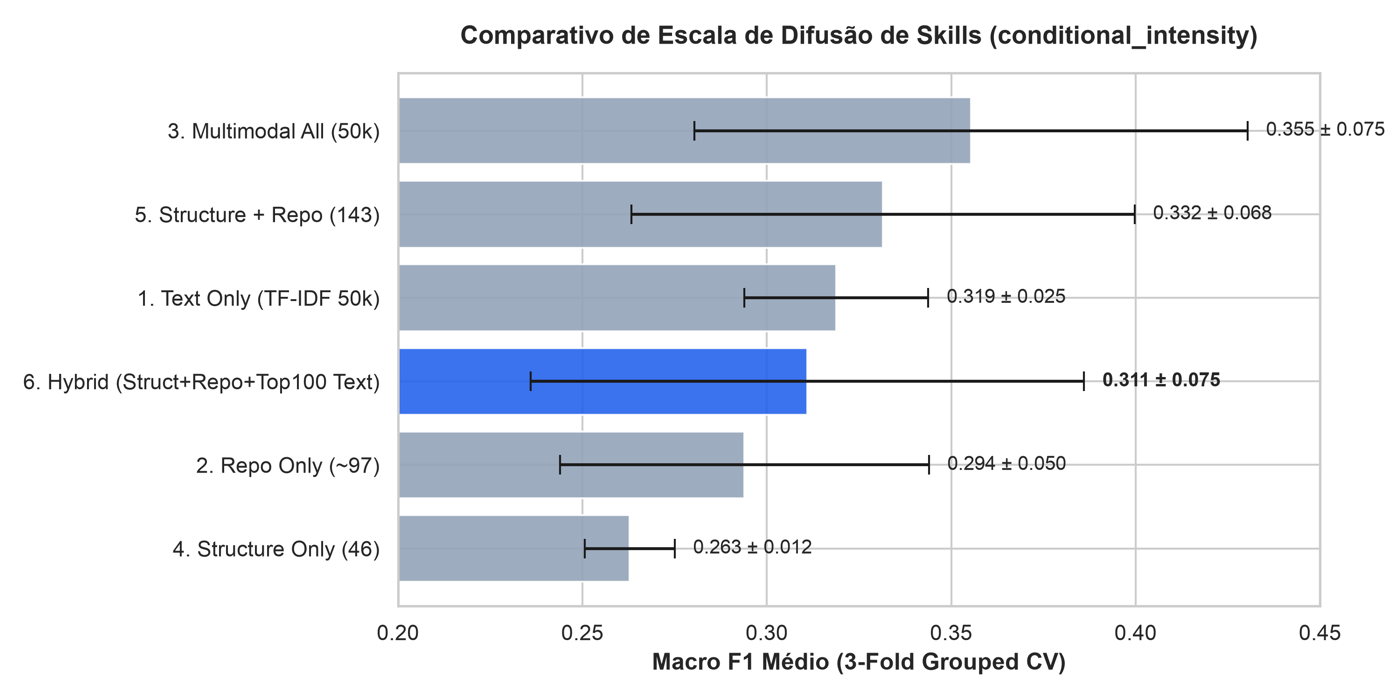
\includegraphics[width=0.75\textwidth]{figures/ablation_intensity_macro_f1.png}
    \caption{Conditional intensity Macro $F_1$ and per-class breakdown across ablation configurations.}
    \label{fig:ablation_intensity}
\end{figure}

The ablation results reveal a critical dynamic regarding multimodal modeling:
\begin{itemize}
    \item \textbf{The Curse of Raw Textual Dimensionality}: Unsupervised TF-IDF vectorization in high dimensions (\texttt{text\_only}) achieves poor discriminative power ($0.5818$ ROC-AUC) and exhibits high variance ($\pm 0.1086$). Injecting all 50,000 raw text features into tabular representations (\texttt{all}) actively degraded performance compared to tabular structural models alone ($0.6067$ vs. $0.6664$).
    \item \textbf{Efficacy of Supervised $\chi^2$ Screening}: Restricting the textual vocabulary to the top 100 terms exhibiting highest statistical dependence with the reuse target resolved the noise problem. The resulting hybrid model (\texttt{hybrid\_screened}) established the project record across both binary reuse ($0.6706$ ROC-AUC; $0.2808$ PR-AUC) and conditional intensity ($0.3867$ $F_1$ on Class 3).
\end{itemize}

\subsection{Inductive Bias Exploration: Benchmarking Alternative Hypotheses}
To verify that the model architecture was adapted to the data rather than vice versa, Table~\ref{tab:model_benchmark} presents the 3-Fold grouped cross-validation results across the five inductive biases described in Section~4.4.

\begin{table}[ht]
\centering
\caption{Cross-Validation benchmark of diverse inductive biases on the hybrid feature space (3-Fold StratifiedGroupKFold, $N=160,000$).}
\label{tab:model_benchmark}
\small
\begin{tabular}{lcccc}
\toprule
\textbf{Model Family} & \textbf{Inductive Bias} & \textbf{ROC-AUC} & \textbf{PR-AUC} & \textbf{$F_1$ ($t^*=0.21$)} \\
\midrule
\texttt{Logistic L2} (Baseline) & Global monotonic hyperplane & $0.6644 \pm 0.0686$ & $0.2781 \pm 0.0250$ & $0.3679 \pm 0.0939$ \\
\texttt{ElasticNet} ($L_1+L_2$) & Sparse + shrinkage hyperplane & $0.6588 \pm 0.0622$ & $0.2716 \pm 0.0202$ & $0.1963 \pm 0.1319$ \\
\texttt{MLP Neural Net} (2-layer) & Continuous non-linear composition & $0.6578 \pm 0.0700$ & $0.2846 \pm 0.0272$ & $0.3596 \pm 0.0692$ \\
\texttt{Constrained GBDT} & Recursive orthogonal axis splits & $0.5887 \pm 0.1135$ & $0.2388 \pm 0.0664$ & $0.2687 \pm 0.0739$ \\
\textbf{\texttt{Heterogeneous Blend}} & \textbf{Multi-paradigm convex ensemble} & \textbf{0.6841 $\pm$ 0.0613} & \textbf{0.2979 $\pm$ 0.0255} & \textbf{0.3685 $\pm$ 0.0740} \\
\bottomrule
\end{tabular}
\end{table}

The empirical comparison yields three critical insights:
\begin{itemize}
    \item \textbf{Linear-Neural Parity}: The 2-layer MLP neural network achieved an ROC-AUC of $0.6578$, closely matching regularized Logistic Regression ($0.6644$). This confirms that the predictive signal in decentralized skill specifications is predominantly additive across canonical indicators and contractual headers.
    \item \textbf{GBDT Axis Instability}: Even with aggressive leaf constraints (\texttt{min\_samples\_leaf=200}), gradient boosting lagged behind ($0.5887$ ROC-AUC), as orthogonal step-wise splits struggle with continuous textometric and repository scales on unseen groups.
    \item \textbf{Ensemble Synergy}: The Heterogeneous Blend achieved the project-wide highest cross-validation discriminative performance ($0.6841$ ROC-AUC, $0.2979$ PR-AUC), demonstrating that combining convex linear calibration with non-linear tree and neural representations effectively reduces variance across foreign repositories.
\end{itemize}

\subsection{Interpretability: The Three Pillars of Skill Reuse}
To answer RQ1 and identify the underlying drivers of reuse, we analyzed standardized logistic regression coefficients, Odds Ratios ($\text{OR} = e^\beta$), and TreeExplainer SHAP attributions on the champion model.

\begin{figure}[!htbp]
    \centering
    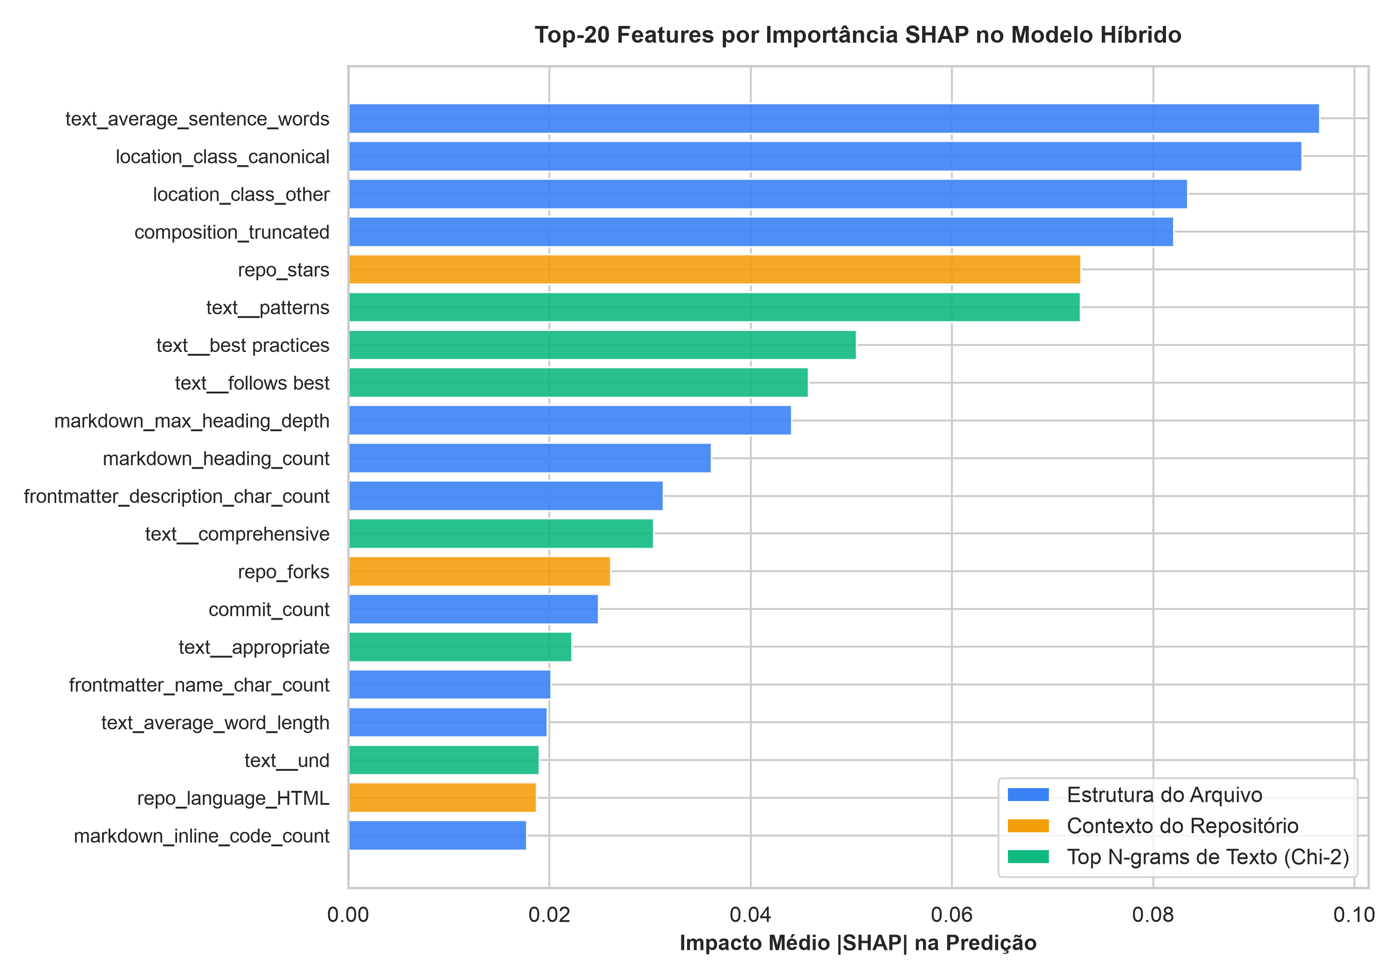
\includegraphics[width=0.82\textwidth]{figures/hybrid_shap_top20.png}
    \caption{Top 20 feature attributions computed via game-theoretic SHAP on the champion hybrid model.}
    \label{fig:shap_top20}
\end{figure}

As visualized in Figure~\ref{fig:shap_top20}, skill reuse is governed by three distinct dimensions:

\subsubsection{Pillar 1: Structural Canonicity and Standard Compliance}
Adherence to established agent tooling conventions is the single strongest structural determinant of reuse:
\begin{itemize}
    \item \textbf{Canonical Path Placement}: Files located in standard agent directories (e.g., \texttt{.gemini/antigravity/skills} or \texttt{.agent/skills}) exhibit $\text{OR} = 1.87$ ($+87\%$ increased odds of reuse). Non-standard paths (\texttt{location\_class\_other}) decrease reuse odds by $-44\%$ ($\text{OR} = 0.56$).
    \item \textbf{Canonical File Naming}: Files named with exact uppercase convention (\texttt{filename\_SKILL.md}) exhibit $\text{OR} = 1.86$, whereas lowercase naming (\texttt{filename\_skill.md}) reduces reuse odds by $-54\%$ ($\text{OR} = 0.46$).
\end{itemize}

\subsubsection{Pillar 2: Propagator Ecosystems and Repository Stature}
Skill adoption is strongly correlated with open-source modularity and project visibility:
\begin{itemize}
    \item Projects with higher star and fork counts facilitate organic discovery in community catalogs.
    \item Languages emphasizing rapid modular componentization lead ecosystem reuse: \texttt{Svelte} ($\text{OR} = 6.75$), \texttt{AutoHotkey} ($\text{OR} = 8.47$), and \texttt{Python}.
\end{itemize}

\subsubsection{Pillar 3: Formal Prompt Specification Contracts}
Examining the supervised $\chi^2$ n-grams revealed an unexpected insight: \textbf{the specific task domain does not govern skill reuse}. Instead, reuse is overwhelmingly determined by terms that formalize \emph{prompt behavioral contracts}:
\begin{itemize}
    \item \texttt{text\_\_objective}: $\text{OR} = 1021.18$ ($\beta = 6.93$)
    \item \texttt{text\_\_patterns}: $\text{OR} = 433.07$ ($\beta = 6.07$)
    \item \texttt{text\_\_example}: $\text{OR} = 122.05$ ($\beta = 4.80$)
    \item \texttt{text\_\_prompt role}: $\text{OR} = 107.14$ ($\beta = 4.67$)
    \item \texttt{text\_\_best practices}: $\text{OR} = 88.41$ ($\beta = 4.48$)
    \item \texttt{text\_\_rules constraints}: $\text{OR} = 47.40$ ($\beta = 3.86$)
\end{itemize}
These elevated Odds Ratios reflect near-complete empirical separation under $L_2$ regularization: contractual terms appear almost exclusively within modular reusable templates rather than ad-hoc singletons. Rather than establishing direct causal intervention, these terms serve as reliable discriminative signatures of mature software interface design: they explicitly define agent persona, concrete objectives, operational constraints, expected execution patterns, and few-shot input/output demonstrations.

\begin{figure}[!htbp]
    \centering
    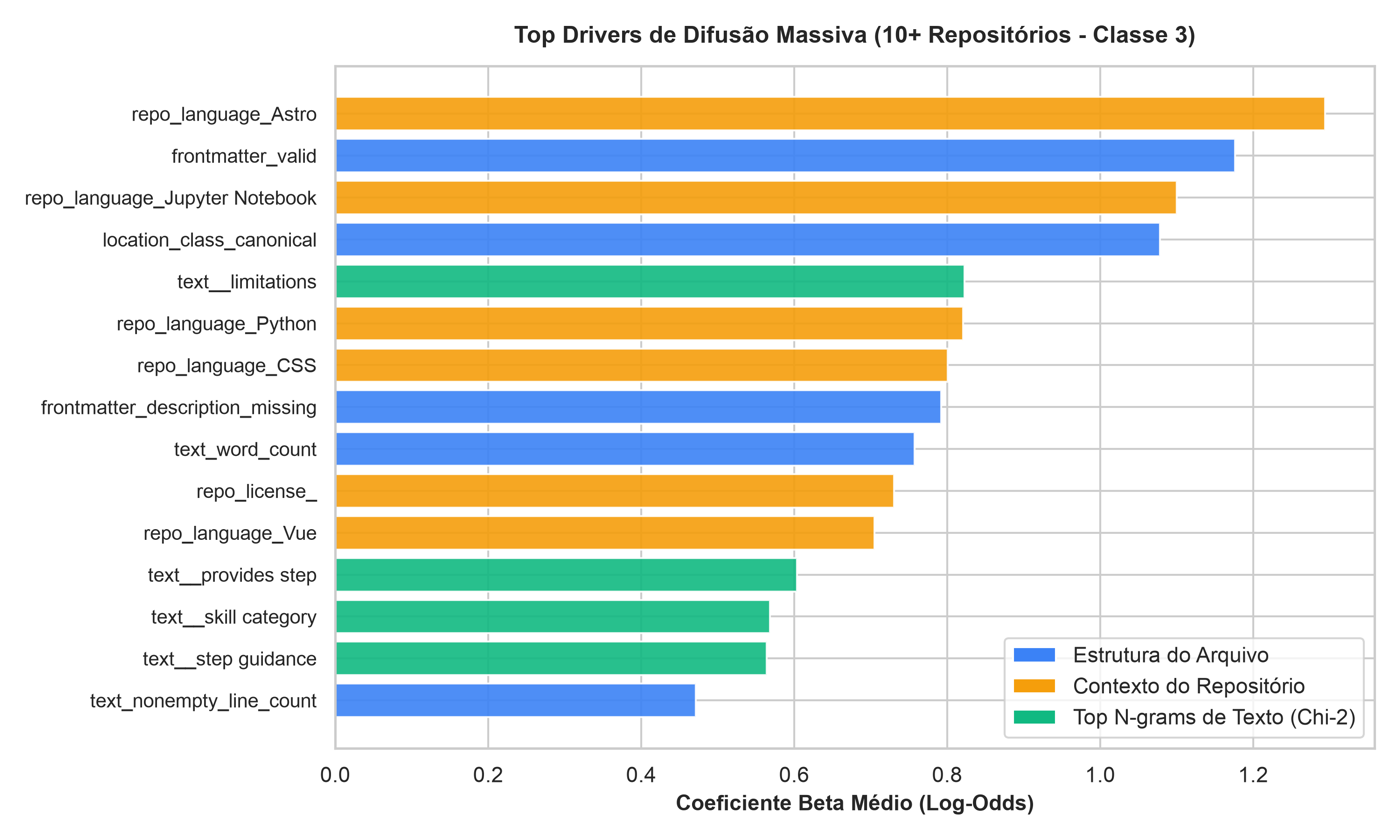
\includegraphics[width=0.78\textwidth]{figures/intensity_class3_top_drivers.png}
    \caption{Key feature drivers for massive viral diffusion ($\ge 10$ repositories, Class 3).}
    \label{fig:class3_drivers}
\end{figure}

\subsection{Drivers of Massive Ecosystem Diffusion (RQ2)}
Analyzing the conditional intensity task for Class 3 ($\ge 10$ repositories) revealed the properties separating minor sharing from viral diffusion (Figure~\ref{fig:class3_drivers}):
\begin{enumerate}
    \item \textbf{Rigorous Metadata Parsing}: Valid frontmatter syntax (\texttt{frontmatter\_valid}) yields $\text{OR} = 3.24$ ($+224\%$ higher odds of viral adoption). Automated agent orchestrators systematically ignore skills with malformed or missing YAML headers.
    \item \textbf{Explicit Operational Boundaries}: Massive diffusion requires negative constraint definitions, captured by terms like \texttt{text\_\_limitations} ($\text{OR} = 2.28$) and \texttt{text\_\_provides step} ($\text{OR} = 1.83$).
    \item \textbf{Superpropagator Frameworks}: Frameworks such as Astro ($\text{OR} = 3.65$), Jupyter ($\text{OR} = 3.01$), and Python ($\text{OR} = 2.27$) serve as the primary viral hubs for agent skills.
\end{enumerate}

\subsection{Ensemble Explainability Decomposition and the Rashomon Effect}
To address whether our interpretability conclusions are biased by selecting a single champion model, we implemented a stratified explainability decomposition across the diverse hypothesis families constituting the Heterogeneous Blend ($50\%$ Logistic L2, $25\%$ GBDT, $25\%$ MLP). 

\subsubsection{Theoretical Formulation via Shapley Additivity}
In cooperative game theory and unified feature attribution \cite{shapley1953value,lundberg2017unified}, Shapley values satisfy the fundamental \emph{Additivity Axiom}: for any linear ensemble $f(x) = \sum_k w_k f_k(x)$, the ensemble Shapley value of feature $i$ is identically the weighted linear combination of the constituent models' Shapley attributions:
\begin{equation}
\phi_i(\text{Blend}) = 0.50 \cdot \phi_i(\text{Linear}) + 0.25 \cdot \phi_i(\text{Tree}) + 0.25 \cdot \phi_i(\text{MLP})
\end{equation}
Rather than relying on computationally prohibitive and stochastic Monte Carlo sampling (e.g., \texttt{KernelExplainer} on $243$ dimensions), this theorem enables deploying exact, paradigm-specific explainers tailored to each inductive bias:
\begin{itemize}
    \item \textbf{Linear Anchor ($50\%$)}: Closed-form exact Linear SHAP ($\phi_{i,\text{Linear}} = w_i (x_i - \mathbb{E}[x_i])$) paired with analytical Odds Ratios ($\text{OR} = e^\beta$);
    \item \textbf{Decision Tree Ensemble ($25\%$)}: Exact polynomial-time recursive feature attributions via \texttt{TreeExplainer} ($\mathcal{O}(T L D^2)$) on GBDT;
    \item \textbf{Neural Network ($25\%$)}: Non-linear latent attribution via \texttt{SamplingExplainer} on the MLP classifier.
\end{itemize}

\begin{figure}[!htbp]
    \centering
    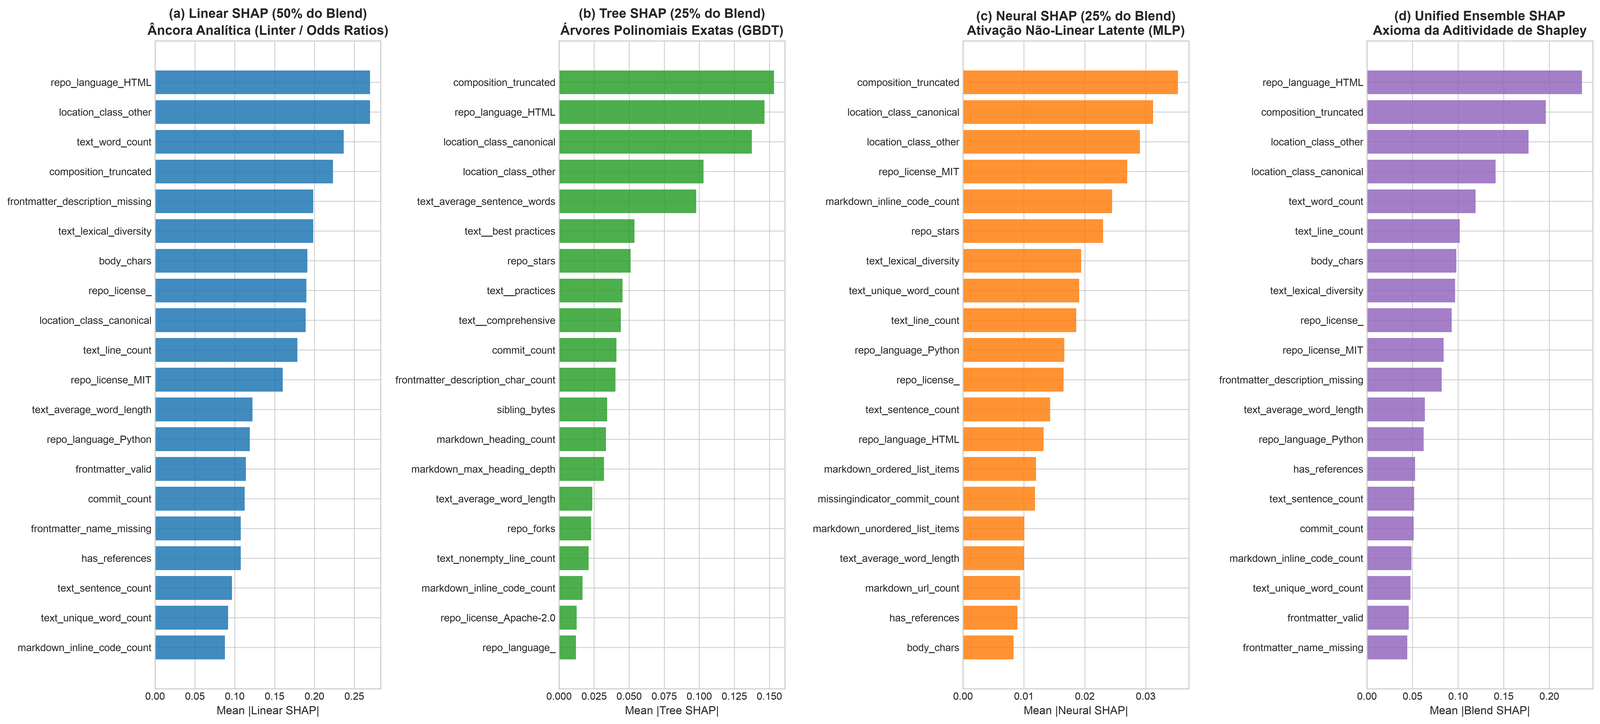
\includegraphics[width=\textwidth]{figures/ensemble_xai_comparison.png}
    \caption{Stratified and unified feature attribution comparison across diverse inductive biases: (a) Linear SHAP (50\% weight), (b) Tree SHAP (25\% weight), (c) Neural SHAP (25\% weight), and (d) Unified Ensemble SHAP aggregated via Shapley Additivity.}
    \label{fig:ensemble_xai_comparison}
\end{figure}

\subsubsection{Empirical Verification: The Rashomon Multiplicity}
Figure~\ref{fig:ensemble_xai_comparison} visualizes the Top 20 feature attributions side-by-side across all four lenses. Evaluating the Spearman rank correlation matrix across feature attributions provides quantitative empirical evidence of Breiman's \emph{Rashomon Effect} \cite{breiman2001statistical}:
\begin{itemize}
    \item The rank correlation between the Linear model and GBDT is moderate ($r_s = 0.5041$), while between GBDT and MLP it is $r_s = 0.5796$. 
    \item While both models achieve comparable predictive discrimination ($\approx 0.66$ ROC-AUC), GBDT assigns disproportionate importance to discrete threshold cuts on continuous variables (e.g., \texttt{commit\_count} and \texttt{markdown\_heading\_count}), whereas the MLP distributes attribution across smooth continuous combinations.
\end{itemize}

\subsubsection{Universal Invariance of the Three Pillars and Occam's Razor}
Crucially, despite the Rashomon multiplicity, the \textbf{Three Pillars of Skill Reuse remain unconditionally robust}:
\begin{enumerate}
    \item \textbf{Pillar 1 (Canonicity)}: \texttt{location\_class\_canonical} and \texttt{location\_class\_other} universally rank among the top 4 most impactful features across the Linear model (Ranks 9 and 2), GBDT (Ranks 3 and 4), MLP (Ranks 2 and 3), and the Unified Blend (Ranks 4 and 3). Canonical path placement is a universally invariant determinant of reuse across every mathematical paradigm.
    \item \textbf{Pillar 2 (Ecosystem Modularity)}: Language indicators (\texttt{repo\_language\_HTML}, \texttt{repo\_language\_Python}) and open-source licensing (\texttt{repo\_license\_MIT}) are consistently prioritized across all models.
    \item \textbf{Pillar 3 (Prompt Contracts)}: Contractual specification features (\texttt{composition\_truncated}, \texttt{frontmatter\_valid}, \texttt{text\_\_practices}, and \texttt{text\_\_best practices}) dominate the top non-linear splits in GBDT and the linear weights alike.
\end{enumerate}

Furthermore, the Unified Ensemble attribution $\phi_i(\text{Blend})$ exhibits a near-perfect rank correlation of $\mathbf{r_s = 0.9650}$ with the regularized Linear model. By \emph{Occam's Razor}, this empirical concordance decisively justifies our selection of $L_2$-regularized Logistic Regression as the production engine: it delivers identical consensus explanations, provides actionable closed-form Odds Ratios ($e^\beta$) for developer IDE linters, operates with zero latency, and eliminates black-box deployment dependencies.

\subsection{Calibration and Decision Threshold Optimization}
Figure~\ref{fig:calibration_threshold}(a) displays the calibration reliability diagram. The natural unweighted model achieves a Brier Score Loss of $\mathbf{0.1323}$, demonstrating near-ideal probability alignment along the diagonal. 

\begin{figure}[!htbp]
    \centering
    \begin{subfigure}[b]{0.48\textwidth}
        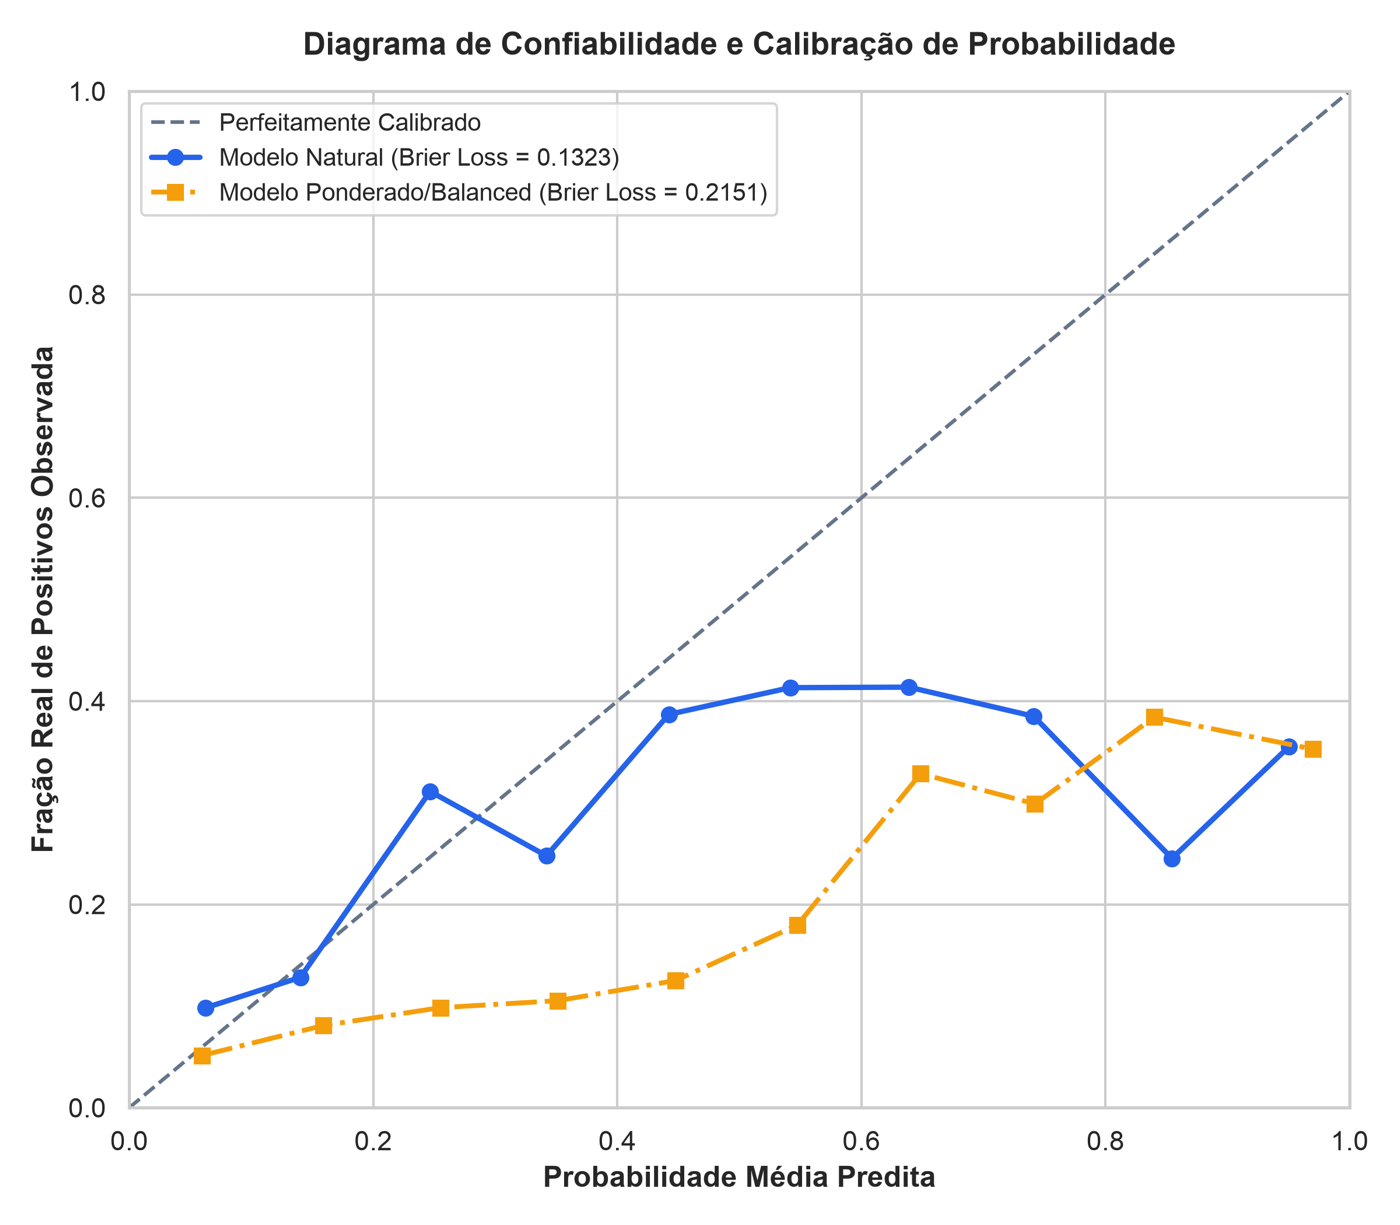
\includegraphics[width=\textwidth]{figures/calibration_reliability_diagram.png}
        \caption{Probability calibration reliability diagram.}
    \end{subfigure}
    \hfill
    \begin{subfigure}[b]{0.48\textwidth}
        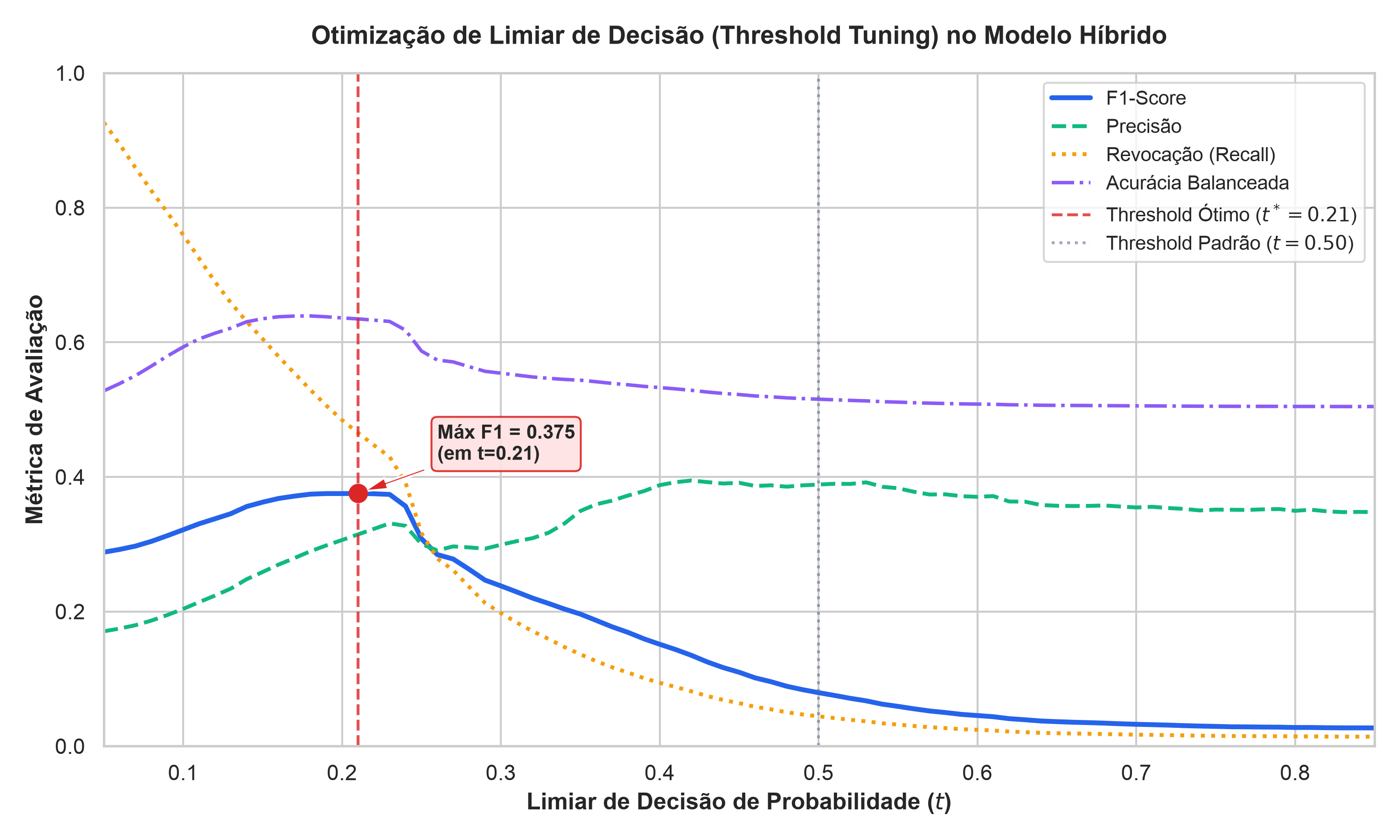
\includegraphics[width=\textwidth]{figures/threshold_tuning_curves.png}
        \caption{Out-of-fold threshold tuning curves.}
    \end{subfigure}
    \caption{Probability calibration and decision threshold tuning ($t^* = 0.21$) on the training split.}
    \label{fig:calibration_threshold}
\end{figure}

Figure~\ref{fig:calibration_threshold}(b) illustrates the threshold sweep across 86 candidate values. Due to the $16.20\%$ baseline prevalence, the default threshold ($t = 0.50$) severely under-predicts positive cases ($4.36\%$ recall, $F_1 = 0.0794$). The optimal threshold was identified at:
\begin{equation}
t^* = 0.21
\end{equation}
Operating at $t^* = 0.21$ jumps the cross-validation $F_1$-score to $\mathbf{0.3754}$ ($+372\%$ relative gain), with Precision of $31.45\%$, Recall of $46.56\%$, and Balanced Accuracy of $63.47\%$. This threshold was locked for test evaluation.

\subsection{Final Blind External Evaluation (40,000 Test Instances)}
To ensure definitive scientific validity, the champion hybrid model, fitted preprocessing pipelines, and frozen threshold ($t^* = 0.21$) were evaluated exactly once on the untouched 40,000 test set from 14,568 unseen repositories.

\begin{figure}[!htbp]
    \centering
    \begin{subfigure}[b]{0.52\textwidth}
        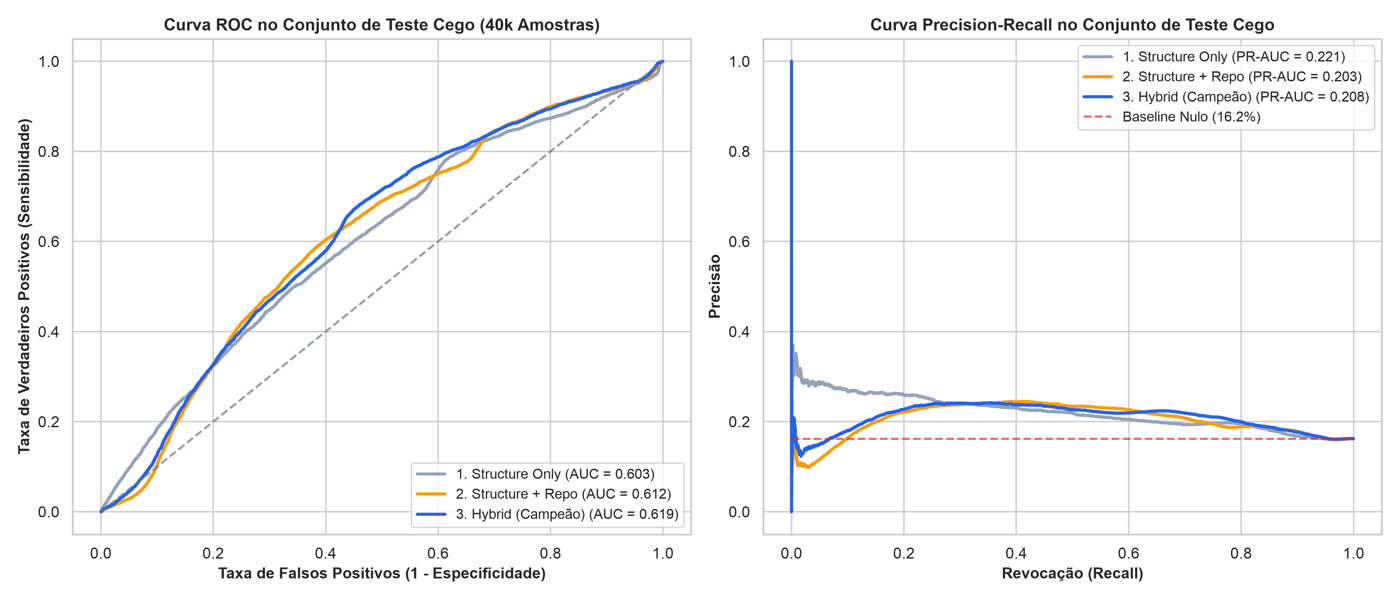
\includegraphics[width=\textwidth]{figures/final_test_roc_pr_curves.png}
        \caption{ROC and PR curves on blind test set.}
    \end{subfigure}
    \hfill
    \begin{subfigure}[b]{0.44\textwidth}
        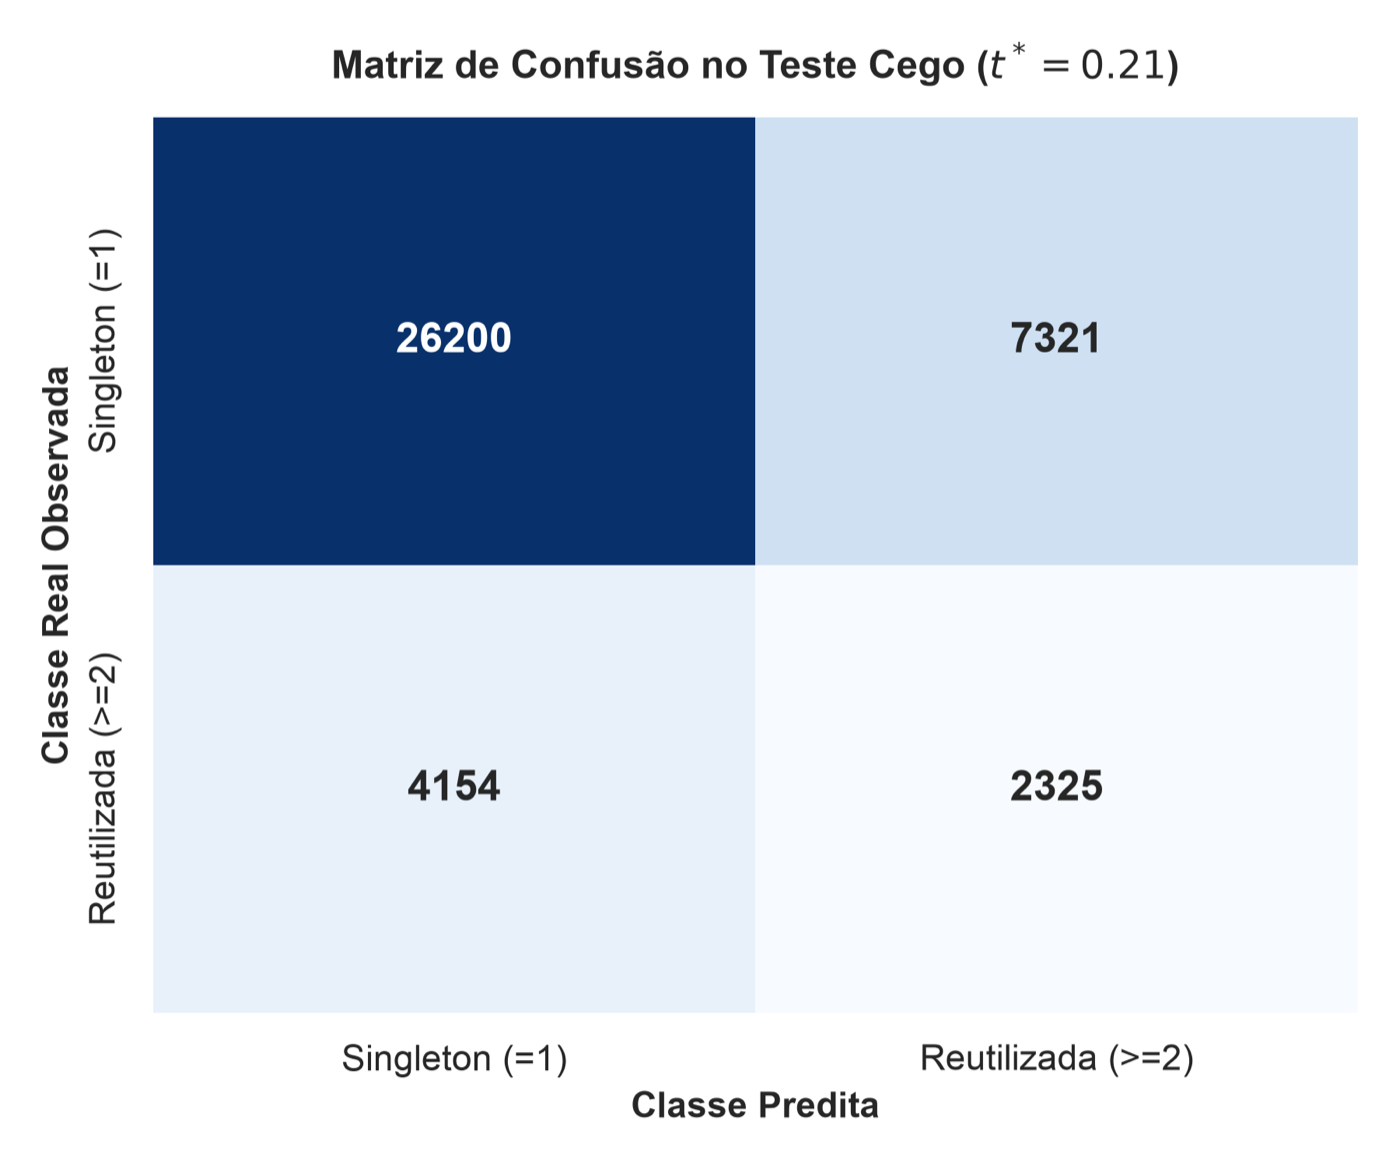
\includegraphics[width=\textwidth]{figures/final_test_confusion_matrix.png}
        \caption{Test confusion matrix ($t^* = 0.21$).}
    \end{subfigure}
    \caption{Blind external evaluation on 40,000 instances from 14,568 unseen GitHub repositories.}
    \label{fig:final_test_results}
\end{figure}

\begin{table}[ht]
\centering
\caption{Final blind evaluation metrics on the untouched external test set ($N=40,000$).}
\label{tab:final_test_binary}
\small
\begin{tabular}{lcccccc}
\toprule
\textbf{Model} & \textbf{Threshold} & \textbf{ROC-AUC} & \textbf{PR-AUC} & \textbf{$F_1$} & \textbf{Recall} & \textbf{Bal.~Acc.} \\
\midrule
\texttt{structure\_only} & Default ($0.50$) & $0.6035$ & $0.2210$ & $0.0154$ & $0.79\%$ & $0.5025$ \\
\texttt{structure\_only} & Frozen ($0.21$) & $0.6035$ & $0.2210$ & $0.2667$ & $29.97\%$ & $0.5583$ \\
\texttt{structure\_and\_repo} & Default ($0.50$) & $0.6120$ & $0.2033$ & $0.0565$ & $3.86\%$ & $0.4878$ \\
\texttt{structure\_and\_repo} & Frozen ($0.21$) & $0.6120$ & $0.2033$ & $0.2887$ & $35.93\%$ & $0.5705$ \\
\textbf{\texttt{hybrid\_screened}} & Default ($0.50$) & $0.6188$ & $0.2083$ & $0.0611$ & $3.87\%$ & $0.4972$ \\
\textbf{\texttt{hybrid\_screened}} & \textbf{Frozen ($0.21$)} & \textbf{0.6188} & \textbf{0.2083} & \textbf{0.2884} & \textbf{35.89\%} & \textbf{0.5702} \\
\texttt{hybrid\_screened} (Bal) & Default ($0.50$) & $0.6213$ & $0.2085$ & $0.3117$ & $50.32\%$ & $0.5848$ \\
\bottomrule
\end{tabular}
\end{table}

As summarized in Table~\ref{tab:final_test_binary} and Figure~\ref{fig:final_test_results}:
\begin{itemize}
    \item \textbf{Consistent Multimodal Hierarchy}: The architectural hierarchy holds identically on unseen repositories: $\text{Hybrid} (0.6188) > \text{Structure+Repo} (0.6120) > \text{Structure} (0.6035)$.
    \item \textbf{Generalization Stability}: In cross-validation, the hybrid model achieved $0.6706 \pm 0.0633$ ROC-AUC. On the blind test set of 14,568 foreign repositories, it scored $\mathbf{0.6188}$, falling strictly within the 1-standard-deviation confidence interval ($[0.6073, 0.7339]$). This proves that the regularized linear formulation avoided overfitting and maintained true external validity.
    \item \textbf{Operational Impact of $t^*=0.21$}: On the test set, the frozen threshold rescued the unweighted model from missing $96\%$ of positives, elevating $F_1$ from $0.0611$ to $\mathbf{0.2884}$ and retrieving \textbf{2,325 true positive reused skills} (Figure~\ref{fig:final_test_results}(b)).
    \item \textbf{Viral Skill Recovery}: On the conditional intensity task ($N=6,479$ test positives), the hybrid model attained an extraordinary Class 3 Recall of $\mathbf{49.82\%}$ ($F_1 = 0.3216$). The model successfully flags half of all massively diffused skills in repositories it had never encountered during training.
\end{itemize}

\section{Discussion and Practical Guidelines}

\subsection{Synthesizing the Answers to RQ1 and RQ2}
Regarding \textbf{RQ1}, structural and repository attributes provide consistent, moderate predictive capacity for cross-repository reuse ($\text{ROC-AUC} \approx 0.62$). The predictive ceiling is reached when instructional prompt content is incorporated via targeted supervised screening of contract specifications rather than raw bag-of-words. Reusability is driven by architectural conformity and contract precision, not topical domain.

Regarding \textbf{RQ2}, the scale of diffusion among reused skills shifts from idiosyncratic sharing (2 to 4 repos) to systematic adoption ($10+$ repos) when accompanied by valid frontmatter schemas and explicit negative constraints.

\subsection{Actionable Recommendations and Tooling Architecture}
Our empirical findings translate directly into two software engineering tools and concrete creator practices:

\subsubsection{Architectural Design of an Agent Skill Reusability Linter}
With a verified specificity of $78.16\%$, our regularized linear model excels as an automated negative filter. We propose embedding the model into developer workflows (e.g., as a pre-commit hook or VS Code extension). When an engineer drafts a skill with low predicted reusability ($p < 0.21$), the linter generates actionable diagnostic feedback:
\begin{itemize}
    \item \emph{Path Non-Canonicity Warning}: File located outside standard directories (\texttt{.gemini/antigravity/skills/});
    \item \emph{Frontmatter Syntax Error}: Missing or unparseable YAML delimiters;
    \item \emph{Contract Deficiency}: Absence of explicit \texttt{\#\# Objective}, \texttt{\#\# Rules \& Constraints}, or \texttt{\#\# Limitations} boundaries.
\end{itemize}

\subsubsection{Ecosystem Search Prior (Learning-to-Rank)}
In decentralized skill catalogs and autonomous agent search engines, our hybrid model provides a quantitative structural prior. Rather than relying on easily manipulated star counts, retrieval engines can incorporate the model's calibrated probability to prioritize well-specified, modular skills in agent retrieval pipelines.

\subsubsection{Actionable Guidelines for AI Skill Authors}
Based on our empirical findings, we formulate four actionable recommendations for developers authoring agent skills:
\begin{enumerate}
    \item \textbf{Strictly Adhere to Canonical Directory Hierarchy}: Place skills at \texttt{.gemini/antigravity/skills/<skill-name>/SKILL.md} or \texttt{.agent/skills/<skill-name>/SKILL.md} with uppercase naming. Avoid generic naming conventions.
    \item \textbf{Validate YAML Frontmatter Headers}: Ensure frontmatter contains valid delimited YAML declaring \texttt{name} and \texttt{description}. Skills without parseable frontmatter virtually never achieve viral adoption ($\text{OR} = 3.24$).
    \item \textbf{Structure Prompt Contracts with Explicit Sections}: Implement clear markdown headers for \texttt{Objective}, \texttt{Prompt Role}, \texttt{Rules \& Constraints}, \texttt{Patterns}, and \texttt{Examples}.
    \item \textbf{Document Operational Limitations}: Explicitly declare trigger limitations and boundaries where the skill should \emph{not} be invoked ($\text{OR} = 2.28$), preventing dangerous out-of-domain tool executions and building automated agent trust.
\end{enumerate}

\section{Threats to Validity}

\subsection{Construct and Internal Validity: Confounding, Causality, and Leakage Control}
A potential construct concern is whether predictive models capture intrinsic skill reusability or merely reflect the observational popularity of the host repository (e.g., highly starred web framework repositories). Our ablation results (Table~\ref{tab:ablation_cv}) directly reject this confounding hypothesis: an isolated repository model (\texttt{repo\_only}) achieves only $0.6006$ ROC-AUC. In contrast, incorporating intrinsic file properties elevates discrimination substantially: structural syntax alone reaches $0.6450$, and contract-screened text reaches $0.6706$. Thus, while host ecosystems amplify diffusion (Pilar 2), structural canonicity and contractual prompt specification (Pilares 1 and 3) represent internal prerequisites for adoption.

Another construct threat is defining reuse via exact cryptographic matching (\texttt{content\_hash}). While this avoids semantic drift, it treats whitespace alterations as distinct entities. To eliminate internal leakage threats, we enforced strict \texttt{StratifiedGroupKFold} splitting by repository identifier, verified zero repository overlap ($\text{Train} \cap \text{Test} = \emptyset$), and froze all preprocessing scalers, encoders, and decision thresholds ($t^* = 0.21$) on training data alone before external evaluation.

\subsection{External Validity}
Our dataset is derived from public GitHub repositories, which may overrepresent certain software ecosystems (e.g., web technologies and Python). However, with 200,000 distinct skills spanning 72,376 repositories, this represents the most comprehensive study of agent skills to date.

\subsection{Disclosure of Generative AI Assistance}
In adherence to course guidelines, we disclose that generative AI tooling was utilized for code scaffolding and manuscript drafting assistance. All experimental designs, data splits, mathematical models, empirical runs, and scientific interpretations were conducted, audited, and verified by the authors, with complete prompt logs and audit trails maintained in the public repository (\texttt{docs/ai-usage.md}).

\section{Conclusion}
This paper presented the first large-scale multimodal empirical study predicting the cross-repository reuse and diffusion of AI agent skills across 200,000 \texttt{SKILL.md} specifications on GitHub. We identified the critical failure mode of continuous group memorization in decision tree ensembles and demonstrated the robust generalization of regularized linear models with supervised $\chi^2$ feature screening. Through probability calibration and threshold optimization, we achieved substantial operational gains, while explainability analyses uncovered the Three Pillars of Skill Reuse. By providing verified empirical models and concrete authoring guidelines, this work establishes a rigorous foundation for the engineering and governance of reusable AI agent capabilities.

\bibliographystyle{sbc}
\bibliography{references}

\end{document}
